\documentclass[border=2mm]{standalone}
\usepackage{pgfplots}
\usepgfplotslibrary{groupplots}
\pgfplotsset{compat=1.18}
\definecolor{BCred}{rgb}{0.7, 0.11, 0.11}
\definecolor{BCblue}{rgb}{0.0, 0.20, 0.42}
\definecolor{BCgreen}{rgb}{0.11, 0.35, 0.02}
\pgfplotsset{every axis/.append style={width=7cm, height=7cm, scale only axis,
  ticklabel style={font=\scriptsize, /pgf/number format/fixed, /pgf/number format/precision=2}, yticklabel style={text width=10mm, align=right}, ylabel style={text width=10mm, align=center}, label style={font=\small},
  title style={font=\small}, legend style={draw=none, font=\footnotesize}}}
\begin{document}
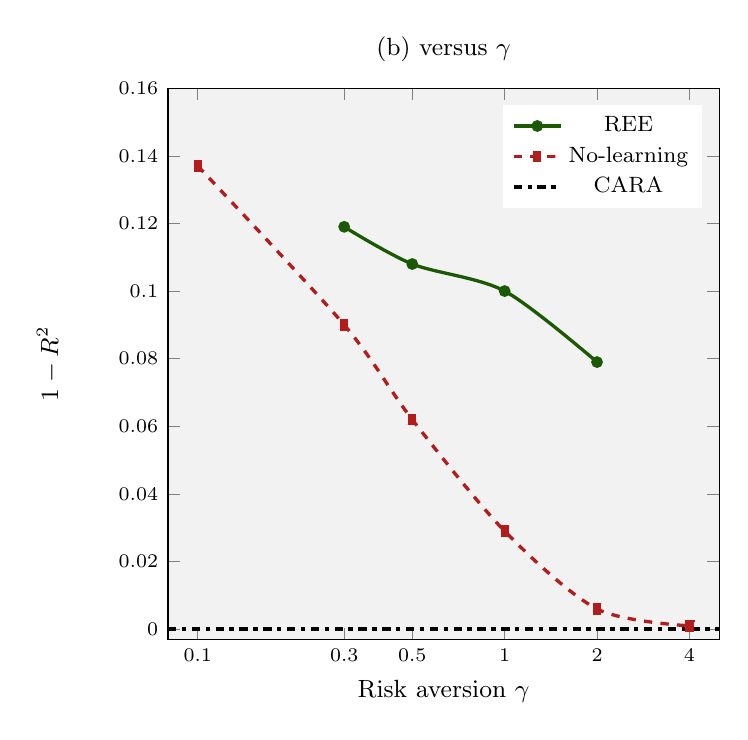
\begin{tikzpicture}
\begin{groupplot}[group style={group size=1 by 1}]
\nextgroupplot[scaled ticks=false,ymin=-0.003, ymax=0.16,
  xmin=0.08, xmax=5, xmode=log,
  xlabel={Risk aversion $\gamma$}, ylabel={$1-R^2$},
  xtick={0.1,0.3,0.5,1,2,4}, xticklabels={0.1,0.3,0.5,1,2,4},
  legend pos=north east, title={(b) versus $\gamma$},
  axis background/.style={fill=black!5}]
\addplot[very thick,color=BCgreen,smooth,mark=*,mark size=1.5pt] coordinates {(0.3,0.119)(0.5,0.108)(1.0,0.100)(2.0,0.079)};
\addplot[very thick,color=BCred,dashed,smooth,mark=square*,mark size=1.5pt] coordinates {(0.1,0.137)(0.3,0.090)(0.5,0.062)(1.0,0.029)(2.0,0.006)(4.0,0.001)};
\addplot[ultra thick,color=black,dashdotted] coordinates {(0.08,0)(5,0)};
\legend{REE,No-learning,CARA}
\end{groupplot}
\end{tikzpicture}
\end{document}
